\chapter{Final Product}

The final product which is implemented is shown in \autoref{fig:designRealFullFinalProduct}. The system has seven stages with different sampling rates. The peak-limiter from \autoref{fig:designRealBlock} is not implemented in the final product. This is due time constraint as there were not enough time to determine the parameter for the limiter.

\begin{figure}[H]
\centering
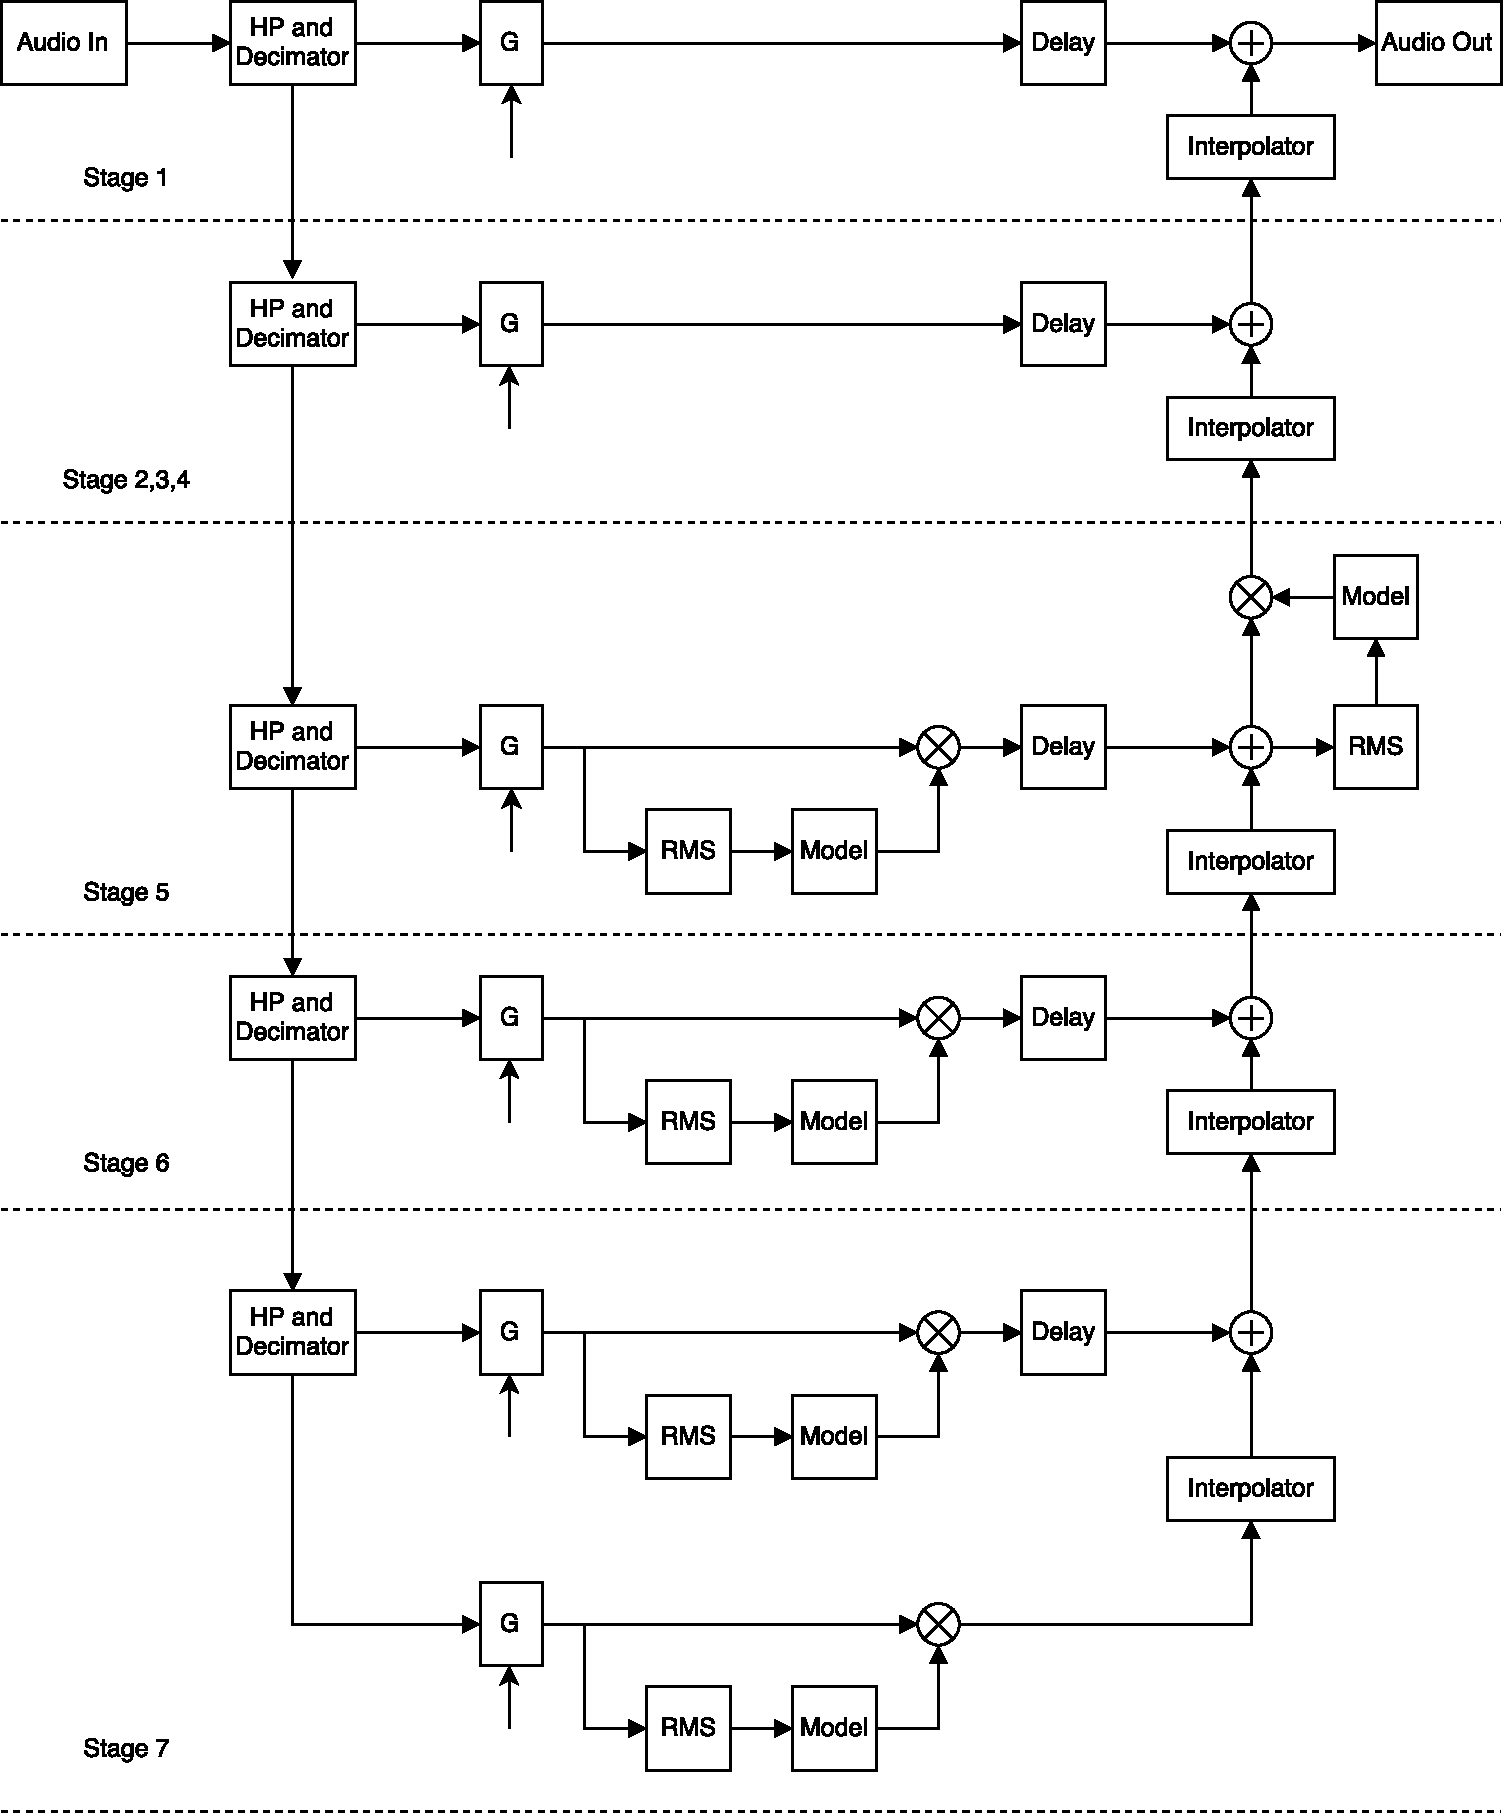
\includegraphics[width=0.75\textwidth]{figures/designRealFullFinalProduct.pdf}
\caption{The block diagram of the final product.}
\label{fig:designRealFullFinalProduct}
\end{figure}

The final product has following features:

\begin{itemize}
\item Volume controller. Volume controller is accessible through the GUI and is able to apply a gain between -42 dB to 0 dB in the system.
\item Eight band equalizer. A gain block is implemented on each band, which can be controlled by the user from the GUI. A gain between -42 dB to 0 dB can be applied in the system.
\item Five RMS limiters where four are implemented into the lowest four octave bands while the fifth limiter is used at the upsampling at stage 5. The RMS limiter protects the loudspeaker against damage by limiting the bass region if the user plays too loud. 
\item Eight band spectrum analyser. A RMS calculator is implemented in each band, and the RMS value in the RMS calculators are then transmitted via UART to the GUI. From the GUI the user can view the RMS value on each band.
\end{itemize}

To verify the implemented features and examine if the system fulfils the requirements, an acceptance test is performed.



